%%%%%%%%%%%%%%%%%%%%%%% file SelHex_proceedings.tex %%%%%%%%%%%%%%%%%%%%%%%%%

\documentclass[proc]{edpsmath}

%%%%%%%%%%%%%--PREAMBLE--%%%%%%%%%%%%%%%%%%
%%-----------------------------
%%         ...........
%%         your macros
%%         ...........
%%-----------------------------
\usepackage{tikz}

%%%%%%%%%%%%%%%--BODY--%%%%%%%%%%%%%%%%%%

\begin{document}
\selectlanguage{english}

%%-----------------------------
%%      the top matter
%%-----------------------------
\title{A semi-Lagrangian solver for the guiding center model on a regular hexagonal mesh}%\thanks{...}\thanks{...}% At most 5 thanks
%
\author{Michel Mehrenberger} \address{IRMA, Universit\'e de Strasbourg, 7, rue Ren\'e Descartes, 67084 Strasbourg \& INRIA-Nancy Grand-Est, projet TONUS, 
\email{mehrenbe@math.unistra.fr}}
\author{Laura S. Mendoza} \address{Max-Planck-Institut f\"{u}r Plasmaphysik, Boltzmannstr. 2, D-85748 Garching, \email{mela@ipp.mpg.de\ \&\ sonnen@ipp.mpg.de}} 
\author{Charles Prouveur}\address{...} %TODO
\author{Eric Sonnendr\"{u}cker}\sameaddress{2}
%
%\dedicated{\it Dedicated to Maurice Dupont} %if necessary
%

\begin{abstract} ... \end{abstract}
%TODO
\begin{resume} ... \end{resume}
%TODO

\maketitle


%%-----------------------------
%%      Introduction
%%-----------------------------
\section*{Introduction}

There are three kinds of regular pavings of the plane: using squares, triangles or hexagons. When considering meshes, the dual mesh of a square mesh is a shifted square mesh and the regular triangle mesh is the dual of the regular hexagonal mesh.

In magnetic fusion applications the embedded magnetic flux surfaces plays an important role and introduces an important anisotropy. For this reason one gets favourable numerical properties when grid points align on the concentric magnetic flux surfaces. When trying to do this with a mapped cartesian grid, one ends up with a polar coordinates mesh (when the flux surfaces are circles) or something topologically equivalent. This yields cells that are smaller and smaller when getting closer to the center and a singularity at the center. This is numerically far from optimal. 

On the other hand tiling a regular hexagon into triangles yields a mesh of equilateral triangles having all the same size, and this can be easily mapped to a circle by slightly stretching the edges of the hexagon. This yields a nice mesh of a disk with slightly stretched triangles of almost the same size and there is no singularity. 
On the other hand such a mesh has a clear structure with three privileged directions, so that it is completely straightforward to localise points within this mesh. On the other hand derivatives along the three directions can be nicely computed using finite differencing along uniform lines. Moreover there is a spline construct on this mesh, called box spline. These splines have a hexagonal support and are invariant by translations along the three directions of the mesh.

%%-----------------------------
%% Interpolation 
%%-----------------------------
\section{Interpolation on regular hexagonal mesh}
%%-----------------------------
\subsection{The hexagonal mesh}

The unit vectors in each direction are

\begin{equation}
	\mathbf{r_1} = \begin{pmatrix}\sqrt{3}/2 \\  1/2
		\end{pmatrix} ~~~~~~~~
	\mathbf{r_2} = \begin{pmatrix}-\sqrt{3}/2 \\ 1/2
		\end{pmatrix} ~~~~~~~~
	\mathbf{r_3} = \begin{pmatrix} 0 \\ 1
		\end{pmatrix}
\end{equation}

The 2D lattice sites are thus obtained by the product $\mathbf{Rk}$ where $\mathbf{R} = [\mathbf{r_1 r_2}]$ and $\mathbf{k} = [k_1, k_2]^T \in \xZ$.  To obtain exactly the mesh as in Figure \ref{fig:hexmesh}, we need to define a few extra parameters : an origin -- denoted $P_0(x_0, y_0)$, a radius $L$ which is the fance between the origin and an external node and the number of cells $N$ on an edge of the exterior hexagon (or in a demi-diagonal).


\begin{figure}[h!]
	\begin{center}
	\begin{tabular}{ccc}
	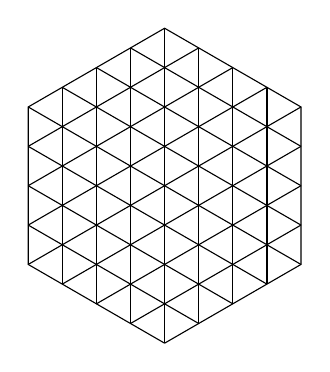
\begin{tikzpicture}
		% Three directions of grid
		% vertical direction
		\draw (0,-2) -- (0,2);
		\draw (-0.433,-1.75) -- (-0.433,1.75);
		\draw (-0.866,-1.5) -- (-0.866,1.5);
		\draw (-1.3,-1.25) -- (-1.3,1.25);
		\draw (0.433,-1.75) -- (0.433,1.75);
		\draw (0.866,-1.5) -- (0.866,1.5);
		\draw (1.3,-1.25) -- (1.3,1.25);

		% upward
		\draw(-1.732,-1) -- (1.732,1);
		\draw (-1.732,-.5) -- (1.3,1.25);
		\draw (-1.732,0) -- (.866,1.5);
		\draw (-1.732,.5) -- (.433,1.75);
		\draw (-1.3,-1.25) -- (1.732,.5); 
		\draw (-0.866,-1.5) -- (1.732,.0);
		\draw (-0.433,-1.75) -- (1.732,-.5);
		% downwards
		\draw(-1.732,1) -- (1.732,-1);
		\draw (-1.732,.5) -- (1.3,-1.25);
		\draw (-1.732,0) -- (.866,-1.5);
		\draw (-1.732,-.5) -- (.433,-1.75);
		\draw (-1.3,1.25) -- (1.732,-.5); 
		\draw (-0.866,1.5) -- (1.732,.0);
		\draw (-0.433,1.75) -- (1.732,.5);
		% Hexagog
		\draw (0,-2) -- (1.732,-1) -- (1.732,1) -- (0,2) -- (-1.732,1) -- (-1.732,-1) -- (0,-2) ; 
	\end{tikzpicture}
	& ~~~~~~~~ &
	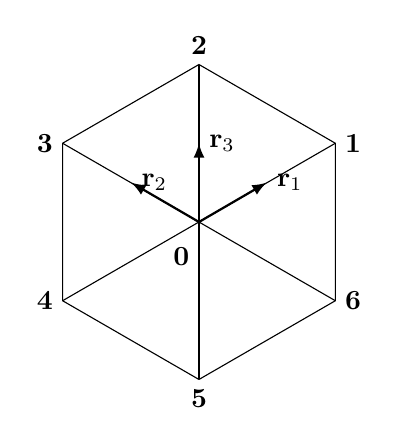
\begin{tikzpicture}
		% Three directions of grid
		% vertical direction
		\draw(0,-2) -- (0,2) node[pos = 0.45, below left]{$\mathbf{0}$};
		\draw[-latex,thick](0,0)--(0,1)node(yline)[right]{$\mathbf{r}_3$};
		\draw[-latex,thick](0,0)--(0.86,.5)node(yline)[right]{$\mathbf{r}_1$};
		\draw[-latex,thick](0,0)--(-0.86,.5)node(yline)[right] {$\mathbf{r}_2$};		
		\draw(-1.732,-1) -- (1.732,1);
		\draw(-1.732,1) -- (1.732,-1);
		\draw (0,-2) node[below]{$\mathbf{5}$} -- (1.732,-1) node[right]{$\mathbf{6}$} -- (1.732,1) node[right]{$\mathbf{1}$} -- (0,2) node[above]{$\mathbf{2}$}-- (-1.732,1) node[left]{$\mathbf{3}$} -- (-1.732,-1) node[left]{$\mathbf{4}$} -- (0,-2) ; % size 2
	\end{tikzpicture}
	\end{tabular}
	\end{center}
	\caption{The hexagonal lattice and the vectors $\mathbf{r_1, r_2, r_3}$ that generate such a mesh}
  \label{fig:hexmesh}
\end{figure}


The mesh is based on uniform hexagons of the first type (see \cite{Ulichney87}). For local and global notations we will use the following convention : the point at the center will be the point of index $0$. Following the direction $\mathbf{r_1}$ the next point will be indexed $1$, and the notations will follow in a counter-clockwise motion for the points on the same ring. And so on, until all the points of the domain have been indexed. See Figure \ref{fig:hexmesh}. We will note $H_i$ the unit hexagon cell that is centred at the point of global index $i$.


%%-----------------------------
\subsection{Box Splines quasi-interpolation}

The accuracy of the Semi-Lagrangian method depends heavily on the interpolation method chosen. For example, for a cartesian grid, it is common to use cubic splines which have shown to give accurate results in an efficient manner. In our problem, with the hexagonal lattice, B-splines don't exploit the isotropy of the mesh (for more information see \cite{Mersereau79-IEEE}) and therefore we need a solution better adapted.  There are mainly two splines families that take advantage of the geometry's properties : hex-splines and the three directional box-splines. For a detailed comparison between these two types of splines we will refer to \cite{Condat2007}. Based on the latter, we have chosen to use box splines.

Let us describe such a model : we are given an initial sample $s[\mathbf{k}] = f_0(\mathbf{R} \mathbf{k})$, where the points $\mathbf{R} \mathbf{k}$ belong to our hexagonal mesh, and we need to know the values $f(X,V)$ where $(X,V) \notin \mathbf{R} \mathbf{k}$. We want a spline surface $f(\mathbf{x}) = \sum c[\mathbf{k}] \chi^n(\mathbf{x} - \mathbf{R}\mathbf{k})$ such that $f(\mathbf{x})$ approximates $f_0(x,v)$ and where $\chi^n$ are the box-splines of compact hexagonal support and $c[\mathbf{k}]$ are the box-splines coefficients which are obtained by \cite{Condat2006a}

\begin{equation}
\label{eqn:coefs}
 c = s * p
\end{equation}

where $*$ is the convolution operator, $s$ is the initial sample data and $p$ is a prefilter which will be defined later on.

\subsubsection{Box-Splines: General Definition}
To construct the box-splines we will use the generator vectors $\mathbf{r_1, r_2, r_3}$ of the hexagonal lattice and we will introduce the box-splines basis functions $\varphi_{\Xi}(\mathbf{x})$ where $\Xi = [\mathbf{v}_1 \mathbf{v}_2]$ which are defined as follows (\cite{Condat2006, Boor1993}):

\begin{equation}
	\varphi_{\Xi} (\mathbf{x}) = \left\{
  	\begin{array}{l l}
    \dfrac{1}{\lvert \det(\Xi)\rvert} & \quad \text{if $\Xi^{-1}\mathbf{x} \in [0,1)^2$ }\\
    0 & \quad \text{otherwise}
  	\end{array} \right.
\end{equation}

and, for higher orders

\begin{equation} \label{eqn:boxsplines_basis}
\varphi_{\Xi \cup [v]}(\mathbf{x}) = \int_0^ 1 \varphi_\Xi(\mathbf{x}-t\mathbf{v})dt
\end{equation}

\subsubsection{Box splines coefficients}

How we determine the splines coefficients is almost as important as the splines themselves. We recall we have the formula \eqref{eqn:coefs}. Based on the literature available (notably \cite{Condat2007}) we have chosen for second-order box-splines the quasi-interpolation pre-filters $p_{IIR2}$ which seem to give the better results within a competitive time. The pre-filter $p_{IIR2}[i]$ of the point of local index $i$, for splines of order 2, is defined as follows : 


\begin{equation}
\label{eqn:filterIIR2}
p_{IIR2} [i] = \left\{
  \begin{array}{l l}
    1775/2304\text{,} & \quad \text{if } i = 0\\
    253/6912\text{,} & \quad \text{if } 0<i<7\\
    1/13824\text{,} & \quad \text{if } 6<i<19 \text{ and $i$ odd}\\
    11/6912\text{,} & \quad \text{if } 6<i<19 \text{ and $i$ even}\\
    0 & \quad \text{otherwise}
  \end{array} \right.
\end{equation}

Or for the splines of order 3 :

\begin{equation}
\label{eqn:filterIIR3}
p_{IIR2} [i] = \left\{
  \begin{array}{l l}
    244301/460800\text{,} & \quad \text{if } i = 0\\
    42269/576000\text{,} & \quad \text{if } 0<i<7\\
    -11809/6912000\text{,} & \quad \text{if } 6<i<19 \text{ and $i$ odd}\\
    1067/144000\text{,} & \quad \text{if } 6<i<19 \text{ and $i$ even}\\
    -23/576000\text{,} & \quad \text{if } 18<i<37 \text{ and ($k_1 = 0$ or $k_2 = 0$ or $k_1 = k_2$) }\\
    -109/288000\text{,} & \quad \text{if } 18<i<37 \\
    	-1/13824000\text{,} & \quad \text{if } 36<i<61 \text{ and ($k_1 = 0$ or $k_2 = 0$ or $k_1 = k_2$) }\\
    	97/6912000\text{,} & \quad \text{if } 36<i<61 \text{ and ($|k_1| = 2$ or $|k_2| = 2$) }\\
    	1/576000\text{,} & \quad \text{if } 36<i<61\\    		
    0 & \quad \text{otherwise}
  \end{array} \right.
\end{equation}

In details, let's give the exact formula for the coefficients. We suppose we have the functions $global(k_1, k_2) = i$ and $local(i,i_0) = j$ that give respectively the global index of $\mathbf{x} = \mathbf{R} \mathbf{k}$ and the local index of that point regarding the point at position $i_0$.

\begin{equation}
c[\mathbf{k}] = \sum_{\mathbf{m} \in \xZ^2} s[\mathbf{m}] \cdot p_{IIR}[local(\mathbf{m} - \mathbf{k}, \mathbf{k})]
\end{equation}

and using \eqref{eqn:filterIIR2} we obtain

\begin{align}
\label{eqn:coef_algo}
c[\mathbf{k}] = \sum_{local(\mathbf{m} - \mathbf{k}, \mathbf{k}) = 0}^{18} s[\mathbf{m}] \cdot p_{IIR}[local(\mathbf{m} - \mathbf{k}, \mathbf{k})]
\end{align}


\subsubsection{Optimizing the evaluation}

For the present state we have all the elements for the approximation of a function $f$ with second order box splines

\begin{equation}
\tilde{f}(\mathbf{x}) = \sum_{\mathbf{k} \in \xZ^2} c[\mathbf{k}] \chi^2(\mathbf{x} - \mathbf{R}\mathbf{k})
\end{equation}

Even if we limit our sum to the vector $\mathbf{k}$ that defines our domain, we would like to take advantage of the fact that the splines $\chi^2$ are only non-zeros in a limited number of points. Therefore we need to know the indices $\mathbf{k}$ such that $\chi^2(\mathbf{x} - \mathbf{R} \mathbf{x}) \neq 0$. For this purpose we will use the strategy suggested in \cite{Condat2007} : to start we need to obtain the indices on the coordinate system generated by $\mathbf{R}$ : $\mathbf{k}_0 = \left[ \lfloor u \rfloor \; \lfloor v \rfloor \right]$ where $\left[ u \; v \right]^T = \mathbf{R}^ {-1} \mathbf{x} $. Thus, in our case, with splines $\chi^2$ we only need 4 terms associated to the encapsulating rhomboid's vertices : $\mathbf{R}\mathbf{k}_0$, $\mathbf{R}\mathbf{k}_0 + \mathbf{R}_1$, $\mathbf{R}\mathbf{k}_0 + \mathbf{R}_2$ and $\mathbf{R}\mathbf{k}_0 + \mathbf{R}_1 + \mathbf{R}_2$. Finally we obtain :

\begin{align}
\label{eqn:chi2_fct_interpol}
\tilde{f}(\mathbf{x}) =& \;\;\;\;\; c[\mathbf{k}_0] \; \chi^2(\mathbf{x} - \mathbf{R}\mathbf{k}_0) \nonumber\\
	&+ c[\mathbf{k}_0 +[1,0]]\; \chi^2(\mathbf{x} - \mathbf{R}\mathbf{k}_0 - \mathbf{R}_1) \nonumber\\
	&+ c[\mathbf{k}_0 +[0,1]]\; \chi^2(\mathbf{x} - \mathbf{R}\mathbf{k}_0 - \mathbf{R}_2) \nonumber\\
	&+ c[\mathbf{k}_0 +[1,1]]\; \chi^2(\mathbf{x} - \mathbf{R}\mathbf{k}_0 - \mathbf{R}_1 - \mathbf{R}_2)
\end{align}

\rmrk  As the $\chi^2$ spline has a support of radius a unity, one of the elements of \eqref{eqn:chi2_fct_interpol} is null. But this formula allow us to keep a short general formula for all points on the mesh without having to compute the indices of the Voronoi cell to which $x$ belongs to.


%%-----------------------------
\subsection{Hermite Finite Elements interpolation}
Another possible way to interpolate is to use a 2d Hermite finite element \cite{zie}   

After the root $(X,V)$ of a characteristic is found and  the triangle in which it is located has been identified... 

There are ten degrees of freedom which are:
\begin{itemize}
\item[-] the values at the vertex of the triangle 
\item[-] the values of the derivatives 
\item[-] the values at the center of the triangle 
\end{itemize}


% mettre un dessin ici des degrés de liberté

\begin{equation}
\begin{cases}  

\partial _x f(x,y) = \partial _{H_1} f(x,y).   \partial _x H_1 +   \partial _{H_2} f(x,y).   \partial _x H_2  \\
\partial _y f(x,y) = \partial _{H_1} f(x,y).   \partial _y H_1 +   \partial _{H_2} f(x,y).   \partial _y H_2             

\end{cases}
\end{equation}

With $H_1$ et $H_2$ the  hexaedric coordinates. Since   

\begin{equation}
\begin{cases}  

\displaystyle{x = \frac{ H_1 - H_2 }{\sqrt{3}} },  \\[2mm]
\displaystyle{y =  H_1 + H_2 },        

\end{cases}
\end{equation}

We obtain :
\begin{equation}
	\begin{cases}  
       \displaystyle{  \partial _x H_1 = \frac{\sqrt{3}}{ 2} ~;~  \partial _y H_1 = \frac{1}{ 2}  }\\[2mm]
       \displaystyle{  \partial _x H_2 = \frac{-\sqrt{3}}{2} ~;~  \partial _y H_2 = \frac{1}{ 2}  } . 
\end{cases}	
\end{equation}

At the vertexes the values are given and $f(G) = \frac{f(S_1)+f(S_2)+f(S_3)}{3}$. As for the values of the derivatives, we use the finite difference method along the hexagonal directions as it can be seen in figure (?)


%%-----------------------------
%% Poisson 
%%-----------------------------
\section{The Poisson equation}
\subsection{Finite Differences Solver}
\subsection{Finite Elements Solver}
\subsubsection{Box-spline basis functions}
\subsubsection{Finite-Element basis functions}


%%-----------------------------
%% BSL
%%-----------------------------
\section{The Backward Semi-Lagrangian Scheme}
\subsection{The Guiding Center Model}
\subsection{General Algorithm}


%%-----------------------------
%% Results
%%-----------------------------
\section{Results}


%%-----------------------------
%%      your bibliography
%%-----------------------------

\newpage
\bibliographystyle{plain}
\bibliography{SelHex_proceedings.bib}

\end{document}

